% Section is about Architecture
% Possibilities - different architectures
% Reasoning over choices - good/bad things about different architectures.
% Choice - the chosen architectures and reasons why
% Description of overall architecture
% Description of application architecture
% Domain model
%%%%%%%%%%%%%%%
% Services
% Possibilities
%%% REST / SOAP
%%% Different frameworks
%%%%% WCF, WEBAPI, etc.
%%% For WCF: Proxies, ABC, protocol choice, Configuration, Serialization
% Reasoning over these - for and against
% choice - and reasons
% How did we use it, and does it work?
% implementation details
%%%%%%%%%%%%%%%%
% Database
% Possibilities 
%%% Why MSSQL Server and not a different technology
%%% ADO.NET vs ORM like entity framework
%%% EF, Code first, TDD, DB-first?
%%%%% Lazy-eager loading?
%%%%% Query generation
%%%%% Pitfalls
% Reasoning over these
% Choice - and reason for choice
% Design of the database, and implementation details and reasoning
% Normalization too
% Relational model
\chapter{Arkitektur}\label{ch:arkitektur}

Dette afsnit omhandler hvilke arkitektur overvejelser der har været i projektet. Da et af målene med projektet er at lave en web-server som kan håndtere samtidighed mellem flere brugere, vil der være bestemte arkitekturer og overvejelser, som kan benyttes til at opnå målet. Herunder Distribuerede Systemer, RESTful Web API, Desktop Programming, Database design og Web design. 

Fremgangsmåden i projektet har været bottom-up, forstået på den måde, at rækkefølgen af hver feature er håndteret i rækkefølgen:
\begin{itemize}\label{procedure}
    \item Database-struktur design (relationel model)
    \item Oprettelse af database tabel(ler)
    \item Design af model (C\#)
    \item Oprettelse af model (C\#)
    \item Oprettelse af DAO
    \item Oprettelse af Controller
    \item Gennemførsel af tests
    \item Simpelt design af front-end
    \item Pænt design af front-end
\end{itemize}

\section{Distribueret System}\label{sec:distSys}
% I need some help explaining better what OSI, TCP/IP, and how all these layers and services relate to that
Dette projekt havde et krav om at være et distribueret system, bestående af flere services, som skulle kunne kommunikere med hinanden gennem en API. API'en er en kontrakt, som sørger for at flere systemer kan kommunikere med hinanden\cite{API}. Dette foregår gennem HTTP protokoller\cite{http}. 
Som navnet "distribueret system" hentyder til, så skal disse services ikke være afhængige af hinanden - de skal decouples\cite{decoupling} og destribueres. Der er flere muligheder når det kommer til design af sådan et system. Det kan designes ud fra en lagdelt arkitektur som OSI eller TCP/IP\cite{osi_tcp}, og gøre brug af MVC design-mønstret. I TCP/IP forekommer disse lag: Applikationslag, Transportlag, Netværkslag og Netværks interface. 
Hvert lag tjener sit eget formål ift. resten af programmet. 
For at gennemføre dette er der blevet brugt en 3-lags arkitektur, som indeholder et præsentationslag, logik lag, og data lag. 

\begin{figure}
    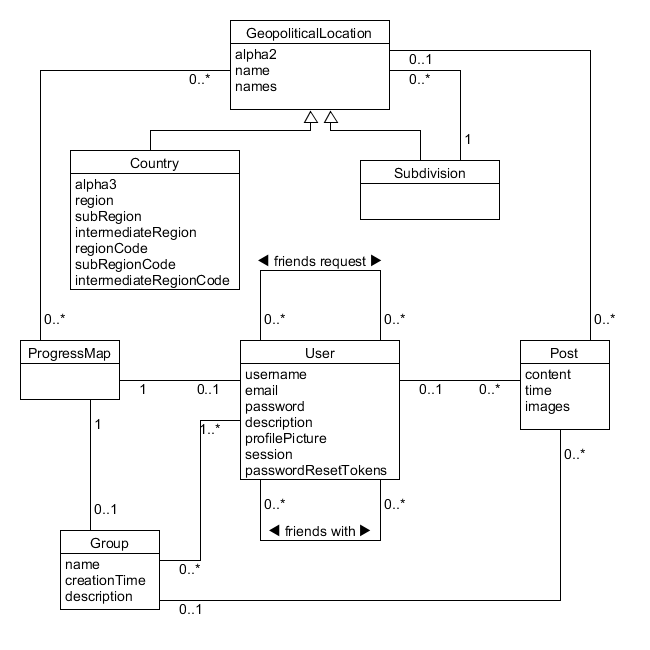
\includegraphics[width=\linewidth]{domain_model.png}
    \caption{QWest domænemodel for databasen.}
    \label{fig:domain_model}
\end{figure}

\subsection{Services}\label{sec:servicesArc}
% Hvilke services benytter vi i QWest?
% Hvilken funktion/ansvar har hver service?
Som nævnt, så bruger man services til at håndtere kommunikation mellem de forskellige dele af programmet. Formålet er at gøre de forskellige dele uafhængige af hinanden så man ikke bare frit kan tilgå databasen, så man kan skjule og ændre back-end uden at påvirke front-end, og centralisere logikken i systemet. 
% Arkitekturen af programmet er struktureret ud fra 3-Tier Architecture\cite{3tier} 
% MVC design mønstret er benyttet

I QWest er der følgende services:
\begin{itemize}\label{services}
    \item QWest.Admin
    \item QWest.Api
    \item QWest.Email
    \item QWest.Web
\end{itemize}

QWest.Admin og QWest.Api er henholdsvis administrator adgang og bruger adgang. QWest.Admin åbner Desktop applikationen, hvor hvert land kan opdateres manuelt. Det skulle så være muligt hvert år at opdatere informationerne på hvert land én gang om året. QWest.Admin benytter sig ikke af Web og Email servicen, da det i dette projekt er vurderet, at det ikke er nødvendigt med front-end til administration. 

\begin{figure}
    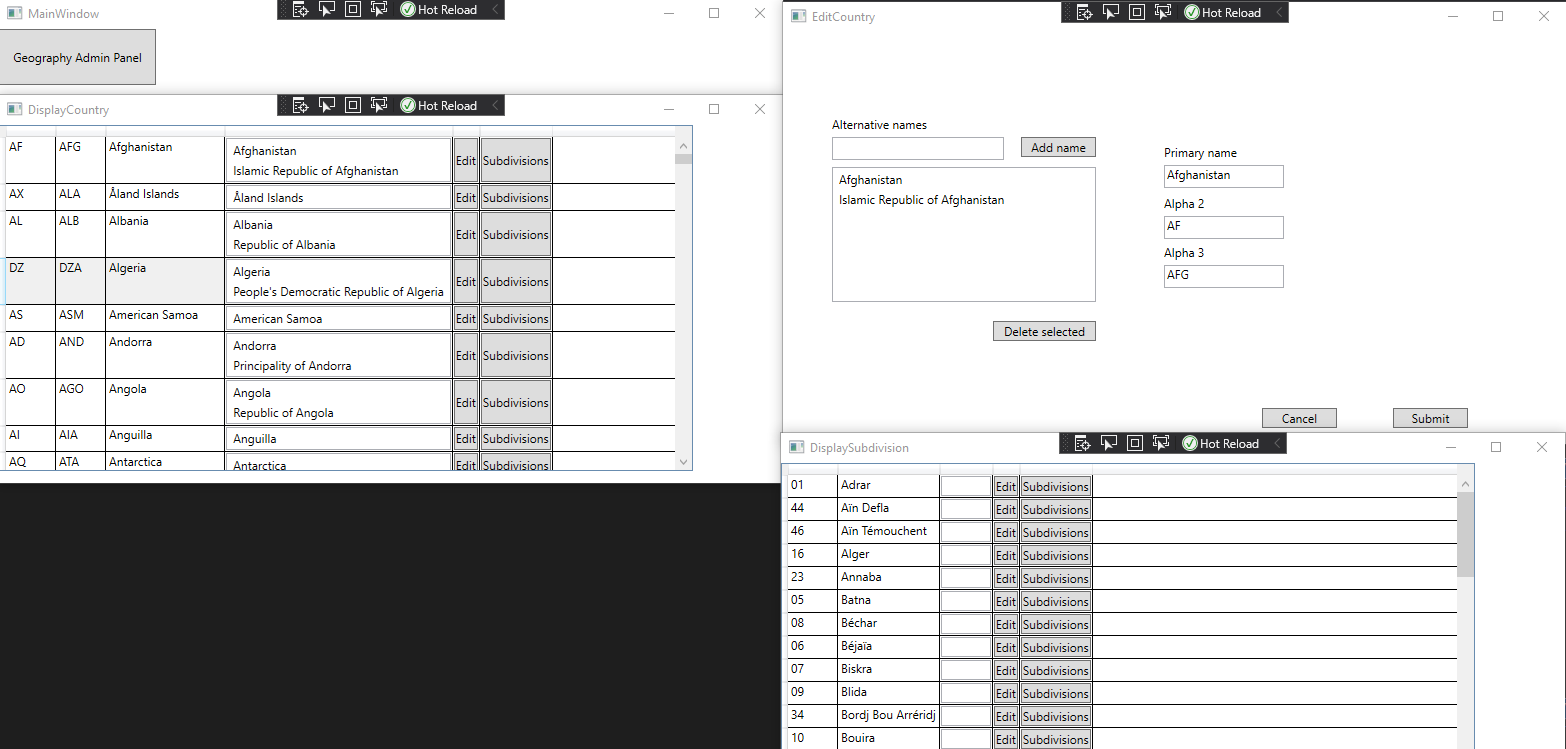
\includegraphics[width=\linewidth]{admin_panel.png}
    \caption{QWest.Admin vinduet, med undervinduer.}
    \label{fig:admin_panel}
\end{figure}

QWest.Api kommunikerer med QWest.Web og QWest.Email. QWest.Email håndterer udsendelse af email til brugeren, såfremt brugeren har bedt om at få sit password nulstillet. QWest.Web er ansvarlig for kommunikation mellem hjemmesiden, model og databasen (gennem QWest.DataAccess).


\section{RESTful Web API}\label{sec:REST}
% Data formats
% Are we working with (SOAP)XML or JSON? 
% WSDL?
% Why chose one over the other; what did you do?

\section{Desktop Programming}\label{sec:deskProgramming}
% This is the QWest.Admin stuff

\section{Database}\label{sec:database}
Databasen til projektet er oprettet med MSSQL\cite{MSSQL}. Til trods for at der findes andre SQL sprog end Microsoft's, blev MSSQL valgt fordi det er det vi i udviklingsteamet kender bedst til. Det ville være risikabelt at bruge en ubestemt mængde af tid på at sætte sig ind i et andet SQL system - især når vi i gruppen allerede har en god forståelse for MSSQL og skolen tildeler en gratis MSSQL server. Til gengæld er der taget højde for, at det skulle være muligt at implementere et andet SQL system - dette er gjort med DAO'er. DAO\cite{dao} designmønstret er gennemgående i projektet og forefindes i koden under QWest.DataAccess. Selve MSSQL implementationen findes i Mssql mappen. 

\begin{figure}
    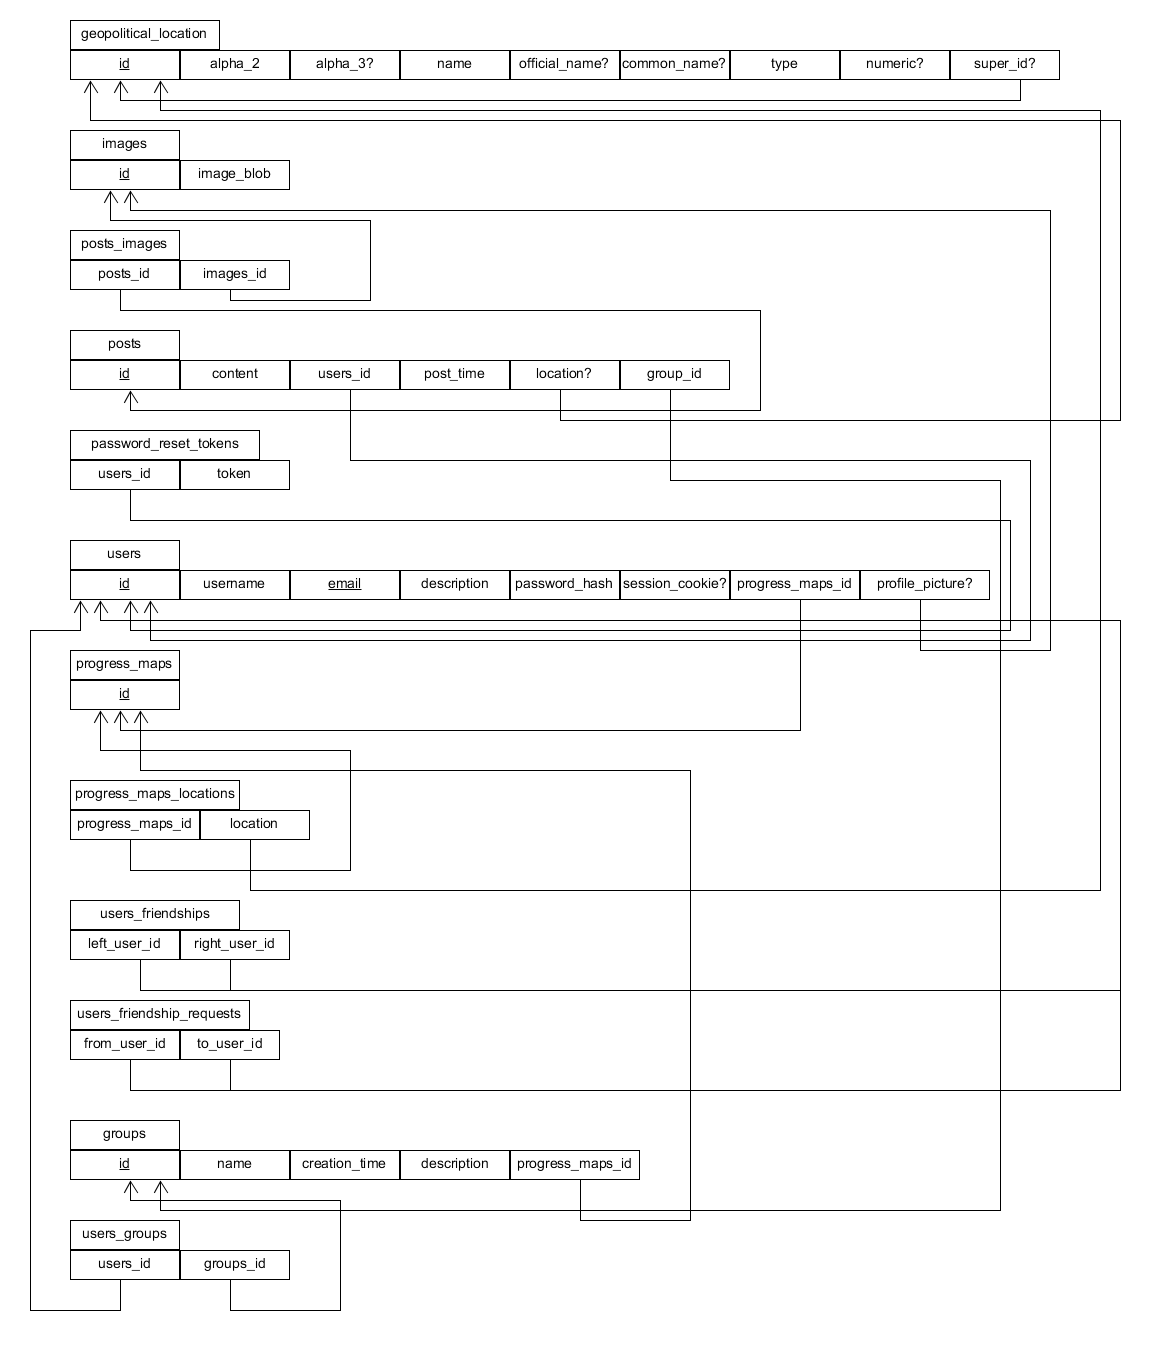
\includegraphics[width=\linewidth]{relational_model.png}
    \caption{QWest relationel model for databasen.}
    \label{fig:relational_model}
\end{figure}

\texttt{users} er omdrejningspunktet i databasen, da \texttt{users} er forbundet med \texttt{progress\_maps}, \texttt{posts}, \texttt{password\_reset\_tokens}, \texttt{users\_friendships}, \texttt{users\_friendship\_requests} og \texttt{users\_groups}. Disse forbinder så til resten af tabellerne, hvor \texttt{posts} har \texttt{posts\_images}, som har \texttt{images}. \texttt{progress\_maps} er forbundet med \texttt{geopolitical\_location}, gennem \texttt{progress\_maps\_locations}. \texttt{groups} er forbundet gennem \texttt{users\_groups}. 
I domæne modellen, figur \ref{fig:domain_model}, ses forholdene mellem klasserne, som er belæg for de forskellige sammenkoblinger af tabellerne så modellerne afspejler hinanden. Databasen opfylder ikke samtlige krav til BCNF\cite{bcnf}. \texttt{name} på \texttt{geopolitical\_locations} og manglen på en seperat \texttt{subregions} tabel til \texttt{geopolitical\_location}. \texttt{name} er ikke atomisk, og kan indeholde flere navne på det samme land. Dette skyldes at lande som regel har flere officielle navne. Eksempelvis kan Storbrittanien hedde "United Kingdom", "Storbrittanien" og "UK", men stadig være det samme på alle andre områder. Såfremt et land har flere officielle navne, så lagres de i ét felt da det beskriver den samme tuple.

%This is probably more important in Implementation than architecture
\section{Web design}\label{sec:webdesign}
\subsection{Back-end and logic}\label{sec:backend}
\subsection{Front-end and usability}\label{sec:frontend}
